\documentclass[12pt]{article}

\usepackage[english]{babel}
\usepackage[utf8]{inputenc}
\usepackage{sansmathfonts}
\usepackage[T1]{fontenc}
\renewcommand*\familydefault{\sfdefault} %% Only if the base font of the document is to be sans serif
\usepackage{multicol,lipsum}
\usepackage{amsmath,cancel}
\usepackage{amssymb,amsthm,dsfont,mathrsfs}
\usepackage[colorinlistoftodos]{todonotes}
\usepackage{geometry}
\geometry{
a4paper,
total={170mm,257mm},
left=20mm,
top=15mm,
bottom=22mm,
}
\usepackage{natbib}
\usepackage{soul}
\usepackage{setspace}
\usepackage{hyperref}
\usepackage{xcolor}
\usepackage{graphicx}
\usepackage{tikz}
\usepackage{siunitx}
\graphicspath{ {imagens/} }
\usepackage{fancyhdr}
\pagestyle{fancy}
\renewcommand{\headrulewidth}{0pt}

\color{darkgray}
\newcommand{\T}[1]{\vspace{0.4cm}\textbf{\large#1}}
\newcommand{\TW}[1]{\textbf{\large#1}}

\newcommand{\TM}[1]{\vspace{0.2cm} \textbf{#1}}

\newcommand{\M}[1]{
\vspace{-0.6cm}
\begin{flalign*}
#1&
\end{flalign*}
\vspace{-0.6cm}
}


\definecolor{bluebell}{rgb}{0.25, 0.35, 0.89} 
\definecolor{laranja}{rgb}{0.87, 0.48, 0.25} 
\definecolor{verde}{rgb}{0, 0.54, 0.44} 
\definecolor{babypink}{rgb}{1, 0.42, 0.52} 
\definecolor{rosa}{rgb}{1, 0.72, 0.77} 
\definecolor{cinza}{rgb}{0.3, 0.3, 0.3}  
\definecolor{iris}{rgb}{0.25, 0.35, 0.89}  
\definecolor{babyblue}{rgb}{0.13, 0.59, 0.95}

\setlength\columnsep{30pt}

\setlength{\parindent}{0cm}
\setlength{\fboxrule}{1.3pt}  % <-- Aumenta a espessura

\newcommand{\Formula}[1]{
\begin{center}
\color{iris}
\fcolorbox{rosa}{white}{
\(
\begin{array}{c}
#1
\end{array}
\)
}
\color{cinza}
\end{center}
}

\begin{document}
\pagenumbering{gobble}
\setstretch{1.3}


\includegraphics[width=4cm]{Logo2.png}
\begin{center}
    \textbf{\Huge \textcolor{bluebell}{Razões Trigonométricas}}
\end{center}

\begin{multicols}{2}

\vspace{0.4cm}
\TW{Descrição} 

As razões trigonométricas relacionam os lados de um triângulo retângulo aos ângulos agudos desse triângulo.  

\begin{center}
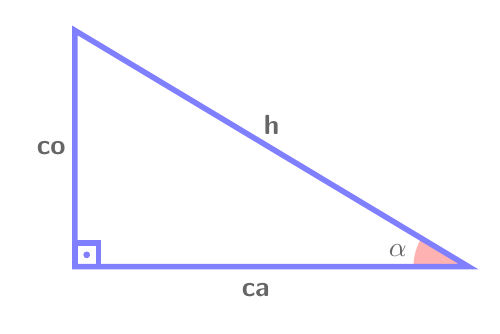
\begin{tikzpicture}
\tikzstyle{texto}=[draw=none,fill=none,black!60!white]
\tikzstyle{line}=[blue!50!white,line width=2pt]
\tikzstyle{angleA}=[draw=none,fill=red!30!white]

\draw[line] (0,0) rectangle (0.3,0.3);
\filldraw[blue!50!white] (0.15,0.15) circle (1pt);

\begin{scope}[shift={(5,0)}]
    \draw[angleA] (0,0) -- (147:0.7) arc (147:180:0.7);
\end{scope}

\draw[line] (0,0) -- (5,0) -- (0,3) -- cycle;

\node[texto] at (4.1,0.2) {\textbf{$\alpha$}};
\node[texto] at (2.5,1.8) {\textbf{h}};
\node[texto] at (-0.3,1.5) {\textbf{co}};
\node[texto] at (2.3,-0.3) {\textbf{ca}};
\end{tikzpicture}
\end{center}

\vspace{-0.2cm}
Nesse triângulo retângulo temos:

-Hipotenusa (h): lado oposto ao ângulo reto.  

-Cateto oposto (co): lado oposto ao ângulo \(\alpha\). 

-Cateto adjacente (ca): ao lado do ângulo \(\alpha\).  

\TM{Seno (sen):}  
\Formula{
sen(\alpha) = \dfrac{\text{cateto oposto}}{\text{hipotenusa}} = \dfrac{co}{h}
}

\TM{Cosseno (cos):}  
\Formula{
\cos(\alpha) = \dfrac{\text{cateto adjacente}}{\text{hipotenusa}} = \dfrac{ca}{h}
}

\TM{Tangente (tan):}  
\Formula{
\tan(\alpha) = \dfrac{\text{cateto oposto}}{\text{cateto adjacente}} = \dfrac{co}{ca}
}

\vspace{-0.2cm}
\TM{Exemplo:}

\begin{center}
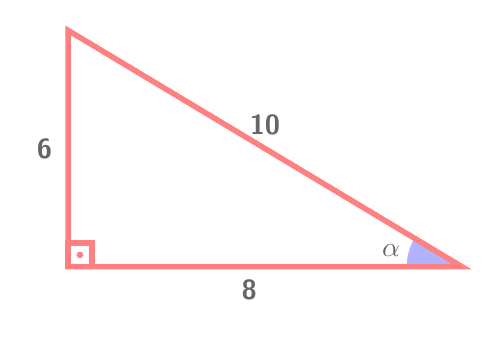
\begin{tikzpicture}
\tikzstyle{texto}=[draw=none,fill=none,black!60!white]
\tikzstyle{line}=[red!50!white,line width=2pt]
\tikzstyle{angleA}=[draw=none,fill=blue!30!white]

\draw[line] (0,0) rectangle (0.3,0.3);
\filldraw[red!50!white] (0.15,0.15) circle (1pt);

\begin{scope}[shift={(5,0)}]
    \draw[angleA] (0,0) -- (147:0.7) arc (147:180:0.7);
\end{scope}

\draw[line] (0,0) -- (5,0) -- (0,3) -- cycle;

\node[texto] at (4.1,0.2) {\textbf{$\alpha$}};
\node[texto] at (2.5,1.8) {\textbf{10}};
\node[texto] at (-0.3,1.5) {\textbf{6}};
\node[texto] at (2.3,-0.3) {\textbf{8}};
\end{tikzpicture}
\end{center}
\[
sen(\alpha) = \dfrac{6}{10} = \dfrac{3}{5}
\]  
\[
cos(\alpha) = \dfrac{8}{10}=\dfrac{4}{5}
\] 
\[
tan(\alpha) = \dfrac{6}{8}=\dfrac{3}{4}
\]  
A seguir apresentamos os principais ângulos notáveis.
%\vspace{-0.5cm}
\begin{center}
\renewcommand{\arraystretch}{1.8} % aumenta 50% o espaçamento das linhas
\begin{tabular}{|c|c|c|c|}
\hline
\textbf{$\alpha$} & \textbf{30°} & \textbf{45°} & \textbf{60°} \\ \hline
\textbf{\textit{sen}}         & $\dfrac{1}{2}$        & $\dfrac{\sqrt{2}}{2}$        & $\dfrac{\sqrt{3}}{2}$        \\ \hline
\textbf{\textit{cos}}          & $\dfrac{\sqrt{3}}{2}$ & $\dfrac{\sqrt{2}}{2}$        & $\dfrac{1}{2}$               \\ \hline
\textbf{\textit{tan}}          & $\dfrac{\sqrt{3}}{3}$ & $1$                         & $\sqrt{3}$                  \\ \hline
\end{tabular}
\end{center}

%\vspace{-0.7cm}
\begin{center}
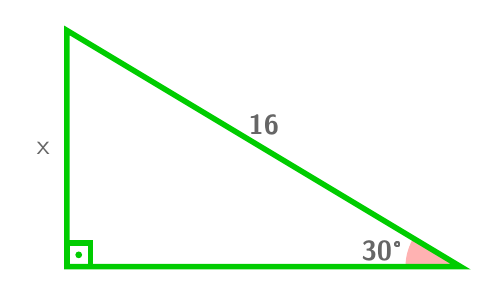
\begin{tikzpicture}
\tikzstyle{texto}=[draw=none,fill=none,black!60!white]
\tikzstyle{line}=[green!80!black,line width=2pt]
\tikzstyle{angleA}=[draw=none,fill=red!30!white]

\draw[line] (0,0) rectangle (0.3,0.3);
\filldraw[green!80!black] (0.15,0.15) circle (1pt);

\begin{scope}[shift={(5,0)}]
    \draw[angleA] (0,0) -- (147:0.7) arc (147:180:0.7);
\end{scope}

\draw[line] (0,0) -- (5,0) -- (0,3) -- cycle;

\node[texto] at (4,0.2) {\textbf{30°}};
\node[texto] at (2.5,1.8) {\textbf{16}};
\node[texto] at (-0.3,1.5) {x};
%\node[texto] at (2.3,-0.3) {\textbf{12}};
\end{tikzpicture}
\end{center}
Utilizando a tabela com os ângulos notáveis, podemos identificar o valor de x por meio do sen 30° $= \dfrac{1}{2}$.

\M{\dfrac{1}{2} &= \dfrac{x}{16}}
\M{2x &= 16}
\M{x &= \dfrac{16}{2}=8}

\end{multicols}
\lfoot{\scriptsize © Copyright, Pratique Já}
\cfoot{\large \textcolor{bluebell}{pratiqueja.com}}
\end{document}